\documentclass[12pt,a4paper]{article}
\usepackage[natbibapa]{apacite}
\usepackage{graphicx}
\usepackage{amsmath}
\usepackage{geometry}
\usepackage{setspace}
\usepackage{enumitem}
\usepackage{hyperref} 
\usepackage{lipsum}
% Page setup
\geometry{margin=1in}
\setstretch{1.5}

% Title Page
\title{Critical Literature Review on [The Role of Artificial Intelligence in Enhancing Software Testing]}
\author{Group Members: \\
\textbf{CHIN ZHEN HO (1221102540)} \\
\textbf{ERIC TEOH WEI XIANG (1221102007)} \\
\textbf{BERNARD RYAN SIM KANG XUAN (1221101777)} \\
\textbf{GAN SHAO YANG (1221103201)} \\
\\
Course: Research Methodologies for Computer Science \\
Assignment 1 - Critical Literature Review \\
Date of Submission: [ 10th September 2024 ]}
\date{}

\begin{document}

\maketitle
\newpage

% Abstract
\begin{abstract}
    \noindent
    [ This literature review investigates the role of Artificial Intelligence (AI) in advancing software testing, with particular emphasis on various AI methodologies, especially Large Language Models (LLMs), and their application in automating and optimizing software testing processes. The review synthesizes insights from four key papers that examine the utilization of LLMs, AI-driven testing tools, and Machine Learning (ML) to address limitations in conventional testing practices. The findings reveal that although AI techniques substantially reduce manual effort and enhance test accuracy, they also introduce new challenges, such as algorithmic uncertainty and the incomprehensibility of models. The review concludes that while AI has the potential to revolutionize software testing, further research is required to fully integrate AI into diverse testing environments and to bridge the existing methodological gaps. ]
\end{abstract}
\newpage

% Table of Contents
\tableofcontents
\newpage

% 1. Introduction
\section{Introduction}
\begin{itemize}
    \item \textbf{Background:} Software development is a human endeavor that involves various activities, including analysis, design, implementation, and testing. Each of these contributes to the creation of the final product, these activities continue in helping with the development process, thus producing a working version of the system can be time consuming.

    As software systems grow more complex and release cycles shorten, the need for efficient and reliable software testing becomes increasingly critical. Traditional manual testing methods are labor-intensive and prone to errors. The advent of AI, particularly LLMs like GPT-3.5 and Codex, offers opportunities to automate various testing tasks, improve accuracy, and reduce the time required for testing, making it a crucial area of research in computer science.

    \item \textbf{Research Problem/Question:}
    How can AI improve the automation and efficiency of software testing, and what are the current trends and challenges in this domain?

    \item \textbf{Objectives of the Review:} The main objectives are to:
    \begin{itemize}
    \item To identify and analyze AI techniques employed in software testing.
    
    \item To assess the effectiveness of AI-driven testing tools.
    
    \item To highlight the challenges and limitations associated with integrating AI in software testing.
    
    \item To suggest directions for future research aimed at improving AI-driven software testing.
    \end{itemize}
    
    \item \textbf{Scope of the Review:} This review encompasses the application of LLMs, AI tools, and ML techniques in automating software testing processes, such as unit test generation, bug detection, and the optimization of testing frameworks. The focus is placed on the use of AI in unit testing, continuous testing, and adaptive testing strategies, while non-AI-based automation techniques are not within the scope of this review.

\end{itemize}

% 2. Literature Review
\section{Literature Review}

\subsection{Overview of Selected Papers}
\begin{itemize}
    \item \textbf{Paper 1:} [An Initial Investigation of ChatGPT Unit Test Generation Capability]
    \begin{itemize}
        \item \textbf{Citation and Authors:} \citep{Guilherme23}
        \item \textbf{Research Focus:}  This study investigates the capability of OpenAI's GPT-3.5-turbo model to generate unit tests for Java programs, benchmarking its performance against established automated testing tools, such as EvoSuite, in terms of test coverage and fault detection.

        \item \textbf{Methodology:} The research involved conducting experiments where GPT-3.5-turbo was tasked with generating unit tests for 33 Java programs. The generated tests were assessed based on their ability to compile, execute without errors, and achieve high code coverage and mutation scores. Variations in test quality was explored by adjusting the model’s temperature parameter to influence the randomness and determinism of the generated outputs.

        \item \textbf{Key Findings:} The study revealed that GPT-3.5-turbo has the potential to generate useful unit tests, though its success was highly dependent on the temperature settings. While the results were promising, the study concluded that large language models, such as GPT-3.5-turbo, are not yet consistently reliable enough to fully replace traditional test generation tools. Instead, they may serve as complementary tools in automated testing frameworks.

    \end{itemize}
    \vspace{0.2cm}
    \item \textbf{Paper 2:} [Automating and Optimizing Software Testing Using Artificial Intelligence Techniques]
    \begin{itemize}
        \item \textbf{Citation and Authors:} \citep{Minimol21}
        \item \textbf{Research Focus:}  This paper investigates the use of Artificial Intelligence (AI) techniques in the software testing process, with the focus being on automation and optimization. It explores how AI can be used to enhance different things of software testing, from different test case generation to detecting whether there are bugs or not, and much more. The paper is aimed at understanding how AI helps to improve the efficiency and effectiveness of testing practices in the development cycle.

        \item \textbf{Methodology:} The research methodology primarily involves a comprehensive literature review. The paper synthesizes findings from various studies on AI-driven software testing, analyzing the implementation of AI tools and techniques across different stages of testing. The author categorizes AI applications in testing into several areas, such as unit testing, integration testing, and user interface (UI) testing, and evaluates the effectiveness of AI-based tools like Selenium, Testim, and Watir. Additionally, the paper discusses AI's role in automating repetitive testing tasks, thus enabling software teams to focus on more complex testing scenarios.

        \item \textbf{Key Findings:} The paper concludes that AI does indeed enhance the testing process by automating routine tasks, improving the accuracy of test results, and reducing the time needed for testing. The author also points out the challenges in integrating AI into traditional testing frameworks, such as needing someone with the skill to manage the AI tools and also the initial setup costs. The paper emphasises the importance of continuous testing, where AI can play a critical role in making sure the software quality is maintained throughout development. Lastly, the study identifies a growing trend towards AI-enabled testing tools that can handle more complex and dynamic testing environments, suggesting a shift in the industry towards more intelligent and adaptive testing solutions.
 

    \end{itemize}

    \vspace{0.2cm}
    \item \textbf{Paper 3:} [LLMs for Intelligent Software Testing: A Comparative Study]
    \begin{itemize}
        \item \textbf{Citation and Authors:} \citep{Boukhlif24}
        \item \textbf{Research Focus:}   This paper investigates the application and effectiveness of Large Language Models (LLMs) in various software testing tasks, particularly in the automated generation of unit tests, metamorphic variables, and test cases. The study aims to compare the performance of different LLMs in these contexts, addressing their strengths and limitations in enhancing software testing processes.

        \item \textbf{Methodology:} This paper conducted a comparative analysis of several LLMs, including Codex, GPT-3, and GPT-J-6B. The study utilised datasets comprising natural language descriptions, source code, and technical documentation as inputs for these models. The evaluation focused on the models' ability to generate test outputs such as unit tests, metamorphic variables, and test cases. Additionally, the effectiveness of prompt engineering and fine-tuning strategies was assessed across different models.

        \item \textbf{Key Findings:}  The study found that while LLMs are capable of generating a diverse range of test artefacts, the quality of these outputs is highly dependent on the model used, the specificity of the input prompts, and the presence of fine-tuning. The research emphasises the crucial role of prompt engineering in producing relevant and high-quality outputs. Moreover, LLMs demonstrate significant potential in automating various aspects of software testing, increasing efficiency, and reducing manual effort.


    \end{itemize}

    \vspace{0.2cm}
    \item \textbf{Paper 4:} [Software Testing: Issues and Challenges of Artificial Intelligence and Machine Learning]
    \begin{itemize}
        \item \textbf{Citation and Authors:} \citep{Kishore21}
        \item \textbf{Research Focus:} This paper explores the unique challenges AI and ML introduce to software testing, particularly focussing on the complexity and unpredictability of these systems. It examines how traditional testing methods fall short when applied to AI/ML models due to issues like data handling, algorithmic uncertainty, and the dynamic nature of these models. The focus is on identifying the gaps in current testing practices and highlighting the need for new strategies that can address the intricacies of AI/ML systems.

        \item \textbf{Methodology:} The authors use a combination of case studies and a comprehensive literature review to analyse the challenges in testing AI/ML systems. They review existing research and real-world applications to understand the difficulties encountered in testing AI/ML models, especially in domains like natural language processing and predictive analytics.

        \item \textbf{Key Findings:} The study concludes that traditional software testing methods are insufficient for AI/ML systems. Major issues include overfitting, where models fail to generalise to new data, and incomprehensibility, where AI decision-making processes are difficult to interpret. The paper advocates for the development of specialised testing frameworks and techniques to better handle the dynamic and complex nature of AI/ML systems.

    \end{itemize}

\end{itemize}

\newpage
\subsection{Critical Analysis of Each Paper}
\begin{itemize}
    \item Evaluate the strengths and weaknesses of each paper
    \begin{itemize}
        \item \textbf{Strengths:} 
        \begin{itemize}
            \item \textbf{Paper 1 :}This paper presents a well-structured empirical analysis, offering valuable insights into how LLMs, specifically GPT-3.5-turbo, can generate unit tests for Java programs. The inclusion of clear metrics, such as code coverage and mutation scores, allows for a quantifiable comparison with traditional tools like EvoSuite. Additionally, it demonstrates the complementary potential of LLMs, suggesting they can enhance, rather than replace current automated testing methods.

            \item \textbf{Paper 2 :} The paper presents a comprehensive overview of AI applications in software testing, offering a well-rounded analysis of current AI tools and techniques. It provides original insights into the integration of AI across various stages of the testing process, particularly in automation. The findings are significant and highly relevant to the ongoing transformation in software engineering, where the importance of automation continues to grow. This combination of thorough analysis, originality, and relevance makes the paper a valuable contribution to the field.

            \item \textbf{Paper 3 :} This paper offers a valuable comparative analysis of various Large Language Models (LLMs) such as Codex, GPT-3, and GPT-J-6B in the context of software testing. The use of diverse datasets, including natural language descriptions and source code, provides a robust basis for evaluating the models’ performance in generating unit tests, metamorphic variables, and test cases. The emphasis on prompt engineering and fine-tuning strategies is a notable strength, highlighting their significant impact on the quality of generated test artifacts.

            \item \textbf{Paper 4 :}  This paper effectively identifies the unique challenges in testing AI/ML systems, such as overfitting and incomprehensibility, highlighting gaps in traditional testing methods. The inclusion of case studies and a comprehensive literature review provides valuable insights and a strong foundation for understanding the specific needs of AI/ML testing, emphasizing the necessity for specialized testing strategies.

        \end{itemize}
        \item \textbf{Weaknesses:} 
        \begin{itemize}
            \item \textbf{Paper 1 :} The study is limited by its focus on a single LLM (GPT-3.5-turbo) and its exclusive use of Java as the testing language. This narrow scope restricts the paper’s applicability to other programming languages and testing scenarios. Furthermore, it does not explore other LLM models or frameworks, limiting its generalizability across different software testing environments.

            \item \textbf{Paper 2 :} The paper could have been better if it had included empirical studies or real-world case examples, as its reliance on secondary data limits the depth of its analysis. The absence of primary research, such as case studies or experimental data, weakens the paper's ability to demonstrate the practical effectiveness of AI tools in diverse software testing environments. By not incorporating original data, the paper misses an opportunity to provide more robust and convincing evidence to support its claims.

            \item \textbf{Paper 3 :} This study's scope is somewhat limited by its focus on a relatively narrow range of LLMs and testing tasks. The paper does not extensively address the qualitative differences in test outputs generated by different models, which could offer deeper insights into their practical utility. Additionally, while the study identifies the importance of prompt engineering, it does not provide a comprehensive analysis of how different fine-tuning methods affect model performance in various testing scenarios.

            \item \textbf{Paper 4 :} The paper primarily focuses on identifying challenges but lacks detailed solutions or actionable strategies to address these issues. This limits its practical application, as it does not provide clear guidance on overcoming the identified challenges. More empirical data could have strengthened its conclusions.
            
        \end{itemize}
        \item \textbf{Relevance: }
            All four papers contribute significantly to understanding AI’s role in software testing, particularly in automating repetitive tasks, generating test cases, and addressing challenges in testing AI/ML systems.
        \begin{itemize}
            \item \textbf{Paper 1 :} This paper is particularly relevant as it investigates the use of Large Language Models (LLMs) like GPT-3.5-turbo for automating unit test generation. By illustrating how LLMs can work alongside traditional tools to generate test cases, it emphasizes AI’s potential in reducing manual efforts and enhancing software testing processes. The empirical data presented further contributes to understanding AI’s role in improving test coverage and fault detection, making it a key reference in the field of AI-driven software testing.
            
            \item \textbf{Paper 2 :} The paper is highly relevant to the research topic of AI's role in enhancing software testing, as it directly addresses how AI techniques can be used to automate and optimize various testing processes. It significantly contributes to the broader understanding of how AI can transform traditional software testing practices, offering valuable insights that can inform both future research and practical applications in the field.

            \item \textbf{Paper 3 :} This paper is highly relevant to the research topic as it explores the application of LLMs in enhancing software testing, directly aligning with the focus on AI-driven techniques. It contributes to understanding how different LLMs can be leveraged to automate and optimize testing processes, thereby supporting the broader goal of improving software testing efficiency and accuracy.

            \item \textbf{Paper 4 :} This paper is highly relevant to the field of software testing, especially for AI and ML applications. As AI/ML systems become more prevalent, traditional testing methods are falling short. The paper’s focus on challenges like overfitting, data handling, and algorithmic unpredictability highlights the need for new testing strategies. It significantly contributes to understanding how AI/ML systems require specialized testing approaches, making it a valuable resource for researchers and practitioners working to ensure the reliability and accuracy of these systems.
            
        \end{itemize}
    \end{itemize}


\end{itemize}

\newpage
\subsection{Comparative Analysis and Synthesis}
\begin{itemize}
    \item \textbf{Themes and Patterns:}  The papers consistently highlight the significant role that AI, particularly LLMs and other AI-driven tools, play in automating routine software testing tasks, such as unit test generation, bug detection, and test case optimization. The recurring theme across all the studies is AI's potential to reduce manual testing efforts while increasing the speed and accuracy of testing processes. However, a common challenge identified is the dependency on prompt engineering and fine-tuning to maximize the utility of LLMs. Another pattern involves the limitations of current AI technologies in handling complex scenarios, particularly in testing AI/ML systems where traditional methods fall short.
    
    \item \textbf{Gaps in the Literature:}There is a noticeable lack of empirical evaluations of AI-driven testing tools across various programming languages and real-world scenarios. Although LLMs and AI tools have shown potential in automating test generation and bug detection, their application in more complex and dynamic environments, such as integration testing, remains underexplored. Furthermore, none of the reviewed studies propose standardized frameworks for evaluating AI tools in testing environments, indicating a gap in the research that could guide future development.

    \item \textbf{Trends:} An emerging trend in the literature is the shift toward AI-enabled continuous testing and the increasing use of LLMs to facilitate unit test generation. Papers also point to the growing integration of AI techniques with traditional testing methods, leading to hybrid approaches. Another trend is the industry’s move toward developing adaptive testing strategies, which allow AI tools to evolve alongside software changes, ensuring sustained quality control.
    
    \item \textbf{Synthesis:} AI is revolutionizing software testing by automating various processes, reducing manual labor, and enhancing accuracy. However, AI-driven tools still face several limitations, such as difficulty in interpreting complex AI/ML systems and the uncertainty surrounding the algorithms they use. Future research should focus on overcoming these barriers by improving AI interpretability, developing new strategies for fine-tuning, and integrating AI more effectively into traditional testing frameworks.


\end{itemize}

\newpage
% 3. Discussion
\section{Discussion}
\begin{itemize}
    \item \textbf{Evaluation of the Literature:} The literature reviewed provides a solid foundation for understanding how AI is transforming software testing. Papers emphasize the potential of AI tools in automating repetitive and time-consuming tasks like unit testing and bug detection. However, the research also underscores the challenges associated with integrating these tools into existing software development workflows. Specifically, the studies identify gaps in current methodologies for testing AI/ML systems and point out the lack of standardized practices for evaluating AI-based testing solutions.
    
    \item \textbf{Gaps in Research:} The key gaps identified in the literature include a lack of real-world evaluations of AI-driven testing tools and insufficient research on testing frameworks tailored for AI/ML systems. While there has been some focus on unit test generation, other critical areas, such as regression and integration testing, remain underresearched. Furthermore, there is little exploration of LLMs beyond those most frequently studied, such as GPT-3 and Codex, leaving out newer models that might offer better performance or additional features.

    \item \textbf{Implications for Future Research:} Future research should aim to address the identified gaps by developing standardized frameworks for evaluating AI-driven testing tools and expanding the focus to include more diverse testing environments. Researchers should also investigate new methods for fine-tuning and prompt engineering to enhance the accuracy and reliability of AI-generated tests. Additionally, the ethical implications of using AI in software testing should be considered, especially as AI-driven testing becomes more prevalent in critical applications.

\end{itemize}

% 4. Conclusion
\section{Conclusion}
\begin{itemize}
    \item \textbf{Summary of Key Findings:} The literature confirms that AI, particularly in the form of LLMs and other AI-driven tools, offers significant advancements in software testing by automating labor-intensive tasks and improving accuracy. However, challenges remain, particularly in dealing with the complexity of AI/ML systems and ensuring that AI-driven testing tools can integrate seamlessly with traditional methods.

    \item \textbf{Reinforce the Importance of the Research Topic:}As software systems become increasingly complex and demand shorter release cycles, the role of AI in enhancing software testing becomes even more critical. AI’s ability to automate testing tasks and improve accuracy has the potential to drastically improve software development efficiency, making this an important area of ongoing research in computer science.
    
    \item \textbf{Suggestions for Future Research:} Future research should focus on real-world evaluations of AI-driven testing tools, exploring how they perform across different environments and programming languages. Additionally, researchers should develop adaptive frameworks that can handle the dynamic nature of AI/ML systems and investigate the ethical considerations of using AI in software testing, particularly in high-stakes applications where accuracy is critical.

\end{itemize}

% References
\newpage
\bibliographystyle{apacite} % Choose the appropriate bibliography style (e.g., APA, IEEE)
\bibliography{MyBib}{} % Make sure to include a MyBib.bib file with your references

% Appendices (if necessary)
\appendix
\section{Appendix A: Member Contributions}
\begin{table}[h]
    \centering
    \begin{tabular}{|c|c|c|}
        \hline
        Student Name & Student ID & Contribution percentages \\
        \hline
        CHIN ZHEN HO & 1221102540 & 25\% \\
        \hline
        ERIC TEOH WEI XIANG & 1221102007 & 25\% \\
        \hline
        BERNARD RYAN SIM KANG XUAN & 1221101777 & 25\% \\
        \hline
        GAN SHAO YANG & 1221103201 & 25\% \\
        \hline

    \end{tabular}
    \caption{Members Contribution Table}
    \label{tab:my_label}
\end{table}

\newpage
\section{Appendix B: [Figure and explanation for The Role of Artificial Intelligence in Enhancing Software Testing]}
\textbf{Paper 1: An initial investigation of ChatGPT unit test generation capability}
\begin{figure}[h]
    \centering
    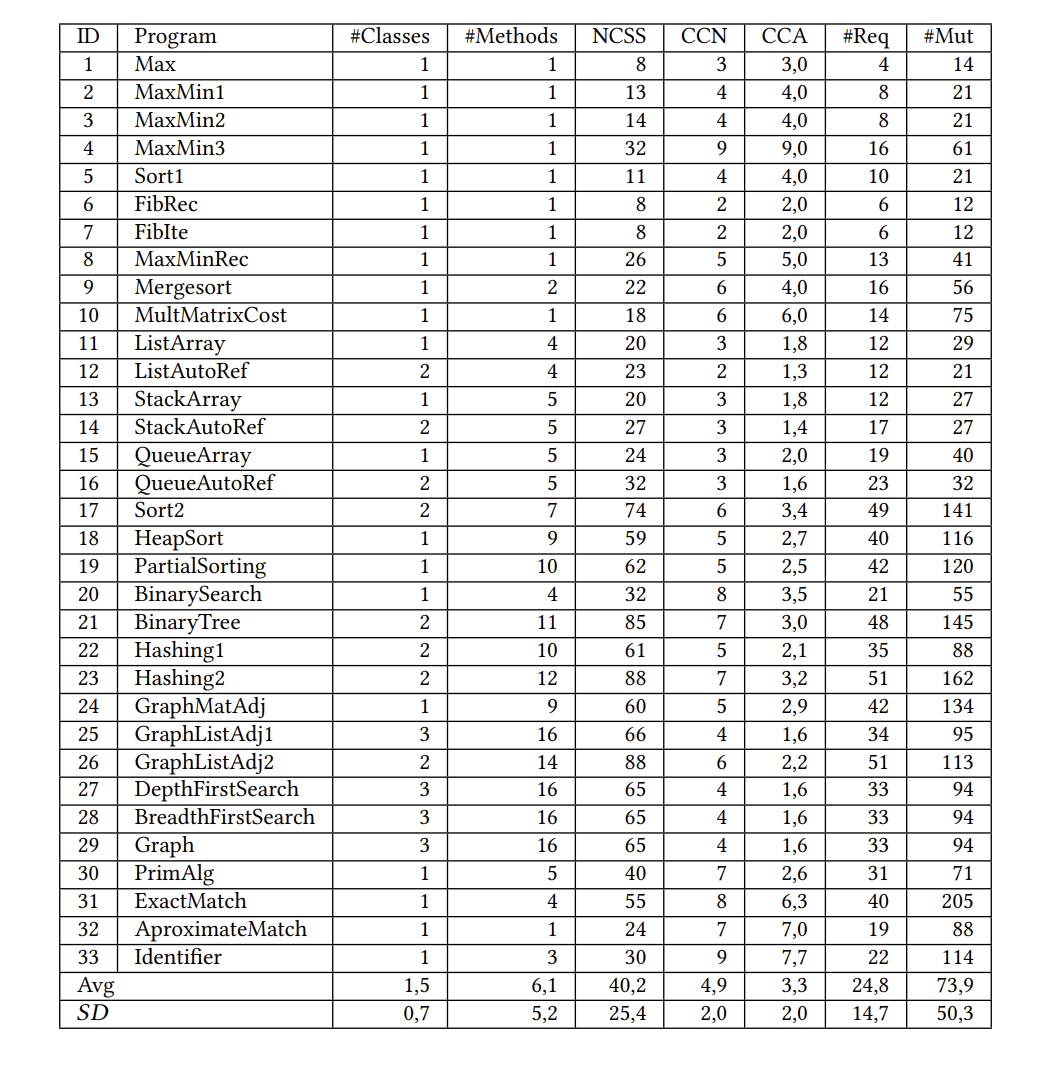
\includegraphics[width=0.8\linewidth]{table1.png}
    \caption{ Static information of the Java programs (extracted from Araujo and Vincenzi [3])}
    \label{fig:enter-label}
    \vspace{0.8em}
    \textbf{Figure 1} provides crucial information about the complexity of the 33 Java programs used in the study. Metrics like Non-Commenting Source Statements (NCSS) and cyclomatic complexity give insight into the size and complexity of the programs. This is important as it sets the context for understanding how the LLM performs on varying codebases, with larger and more complex programs posing greater challenges.
\end{figure}

\begin{figure}[h]
    \centering
    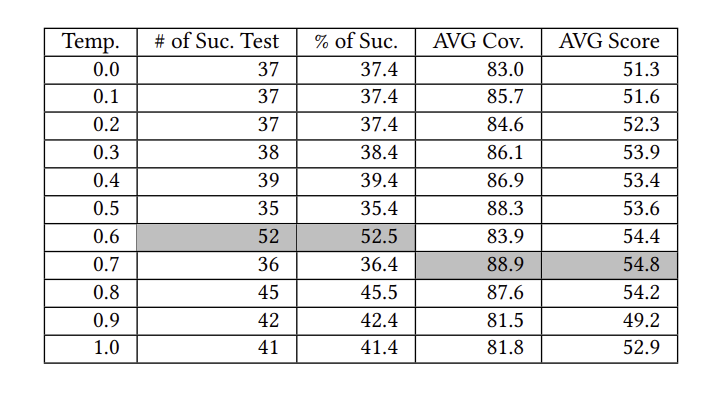
\includegraphics[width=0.5\linewidth]{table2.png}
    \caption{  Average Data for Each Temperature Parameter – Prompt version 1}
    \label{fig:enter-label}
    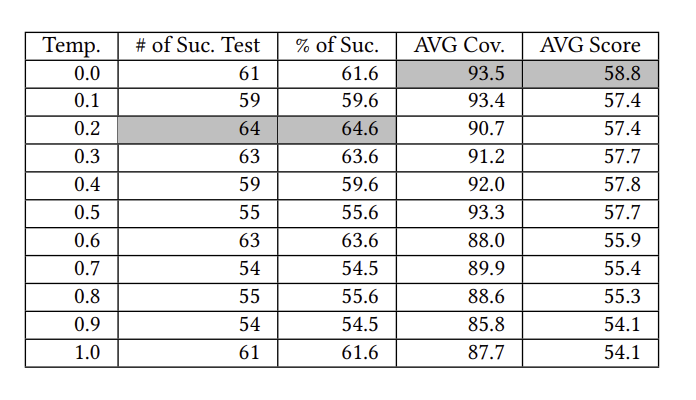
\includegraphics[width=0.5\linewidth]{table3.png}
    \caption{  Average Data for Each Temperature Parameter – Prompt version 2}
    \label{fig:enter-label}
    \vspace{1em}
    \textbf{Figure 2 and 3} present the performance of GPT-3.5-turbo in generating unit tests at different temperature settings, showing key metrics like the number of successful test sets, code coverage, and mutation scores. These tables reveal that lower temperature values resulted in more reliable tests, while higher temperatures introduced more randomness, sometimes reducing effectiveness. Together, these tables illustrate how temperature affects test generation quality and reliability.\\
    \vspace{2em}
    \text The combination of Figure 1, Figure 2, and Figure 3 provides a comprehensive view of the experiment. Figure 1 gives context about the complexity of the programs being tested, while Figure 2 and 3 illustrate how different temperature settings influence the performance of GPT-3.5-turbo in generating unit tests. Together, these tables offer valuable insights into the capabilities and limitations of LLM-based automated test generation, highlighting key areas where GPT-3.5-turbo succeeds and where further improvement is necessary.
\end{figure}

\newpage
\begin{figure}[h]
    \textbf{Paper 2: Automating and Optimizing Software Testing using Artificial Intelligence Techniques}
    \centering
    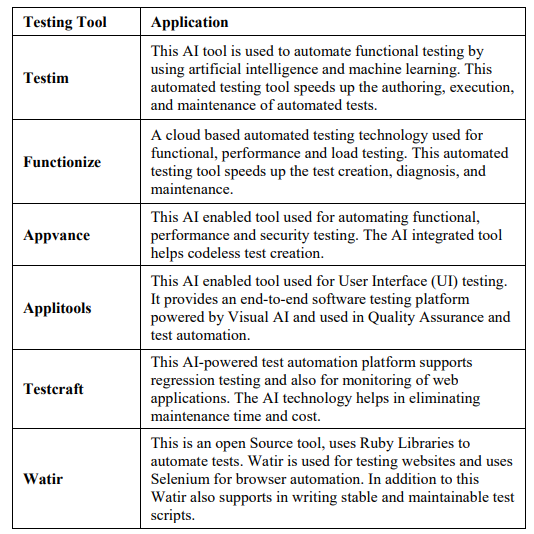
\includegraphics[width=0.8\linewidth]{testingtools.png}
    \caption{Testing Tools}
    \label{fig:enter-label}
    \vspace{0.8em}
    \textbf{Figure 4} shows a summary of several AI-based testing tools and their specific applications in the software testing process. The table highlights tools such as Testim, Functionize, Appvance, Applitools, and Testcraft, each of which leverages AI to automate various testing activities. These tools are designed to enhance different aspects of software testing, from functional testing to UI testing and performance testing.
\end{figure}



\newpage
\begin{figure}[h]
    \textbf{Paper 3 : LLMs for Intelligent Software Testing: A Comparative Study}[h]
    \centering
    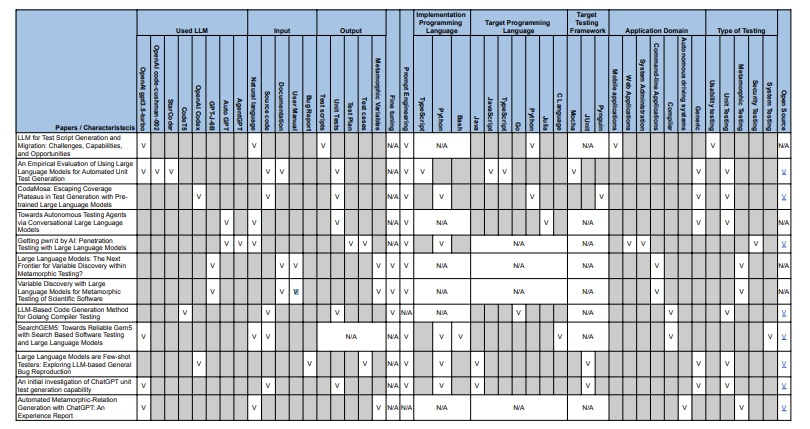
\includegraphics[width=0.8\linewidth]{pic1.jpg}
    \caption{ Comparison between the papers}
    \label{fig:enter-label}
    \vspace{0.8em}
    \textbf{Figure 5} explains the methodology through its inputs and outputs columns. These include inputs like natural language, source code, and user manuals, and outputs like test cases, unit tests, test scripts, and metamorphic variables.Additionally, the table highlights whether prompt engineering was used, which is an important part of fine-tuning the LLMs' performance, supporting the methodological focus on evaluating LLMs based on these criteria.
\end{figure}



\newpage
\begin{figure}[h]
    \textbf{Paper 4 : Software Testing: Issues and Challenges of Artificial Intelligence and Machine Learning}[h]
    \centering
    
\includegraphics[width=0.8\linewidth]{Generalized model.png}
    \caption{ Generalized model}
    \label{fig:enter-label}
    \vspace{0.8em}
    \textbf{Figure 6} shows a well-trained model that performs well on the test data. The red "x" and "0" in the figure represent the error points of the model on the test data. Although the model cannot perfectly predict every data point (there is some error), it captures the overall trend of the data well. This model has moderate complexity and a relatively smooth curve, avoiding overfitting to the training data, so it can perform well on unseen data.
\end{figure}

\begin{figure}[h]
    \centering
    
\includegraphics[width=0.5\linewidth]{Overfit model.png}
    \caption{  Overfit model}
    \label{fig:enter-label}
    \vspace{1em}
    \textbf{Figure 7} shows an overfit model. It performs extremely accurately on the training data and fits every training data point almost perfectly, but the problem is that this complex curve is just "memorizing" the noise of the training data. When the model encounters new data (indicated by the blue question mark in the figure), its predictions may be wrong because the model cannot generalize to situations outside the training data. Although the error of the overfit model on the training data is small, the performance will drop sharply on the test data or actual application.\\
    \vspace{2em}
    \text The model shown in Figure 6 is more accurate because it balances the performance of training data and test data well and avoids overfitting. Although there is a small amount of error, it can generalize to unseen data and provide more stable predictions. The overfit model in Figure 7 performs perfectly on the training data, but performs poorly on new data, indicating that it is too complicated to effectively cope with real-world data changes. Therefore, the model in Figure 6 is more reliable in practical applications.

    
\end{figure}

\end{document}

